\newpage
\mysection{Binary Search Trees}


\begin{figure}[h]
 \centering
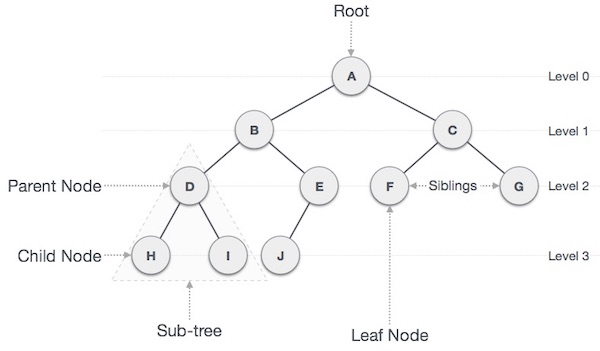
\includegraphics[scale=.6]{images/binary_tree.jpg}
\end{figure}

\mysubsection{Delete}

\mysubsubsection{Case 1: Zero Children}

Deleting a node with no children: remove the node from the tree.

\begin{figure}[h]
 \centering
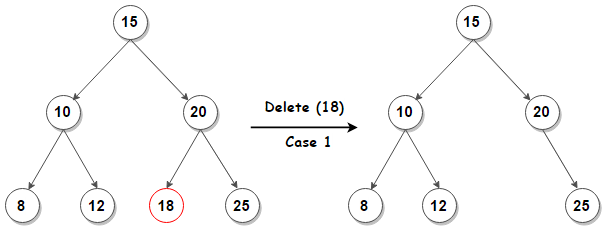
\includegraphics[scale=.6]{images/Deletion-in-BST-Case-1.png}
\end{figure}

\mysubsubsection{Case 2: Two Children}

Find the node to be deleted \textbf{N}. Do not delete \textbf{N}. Instead, choose either its  \lowercase{\gls{inordersucc}} node or its \gls{inorderpred} node, `R`. Copy the value of `R` to `N`, then recursively call delete on `R` until reaching one of the first two cases. If we choose the inorder successor of a node, as the right subtree is not NULL (our present case is a node with 2 children), then its inorder successor is a node with the least value in its right subtree, which will have at a maximum of 1 subtree, so deleting it would fall in one of the first 2 cases.


[inorder](https://www.techiedelight.com/inorder-tree-traversal-iterative-recursive/)